\documentclass[border=10pt]{standalone}

\usepackage{tikz}
\usepackage{tikzsymbols}
\usetikzlibrary{calc,patterns,shapes.geometric}

\def\centerarc[#1](#2)(#3:#4:#5){\draw[#1] ($(#2)+({#5*cos(#3)},{#5*sin(#3)})$) arc (#3:#4:#5);}

\begin{document}
	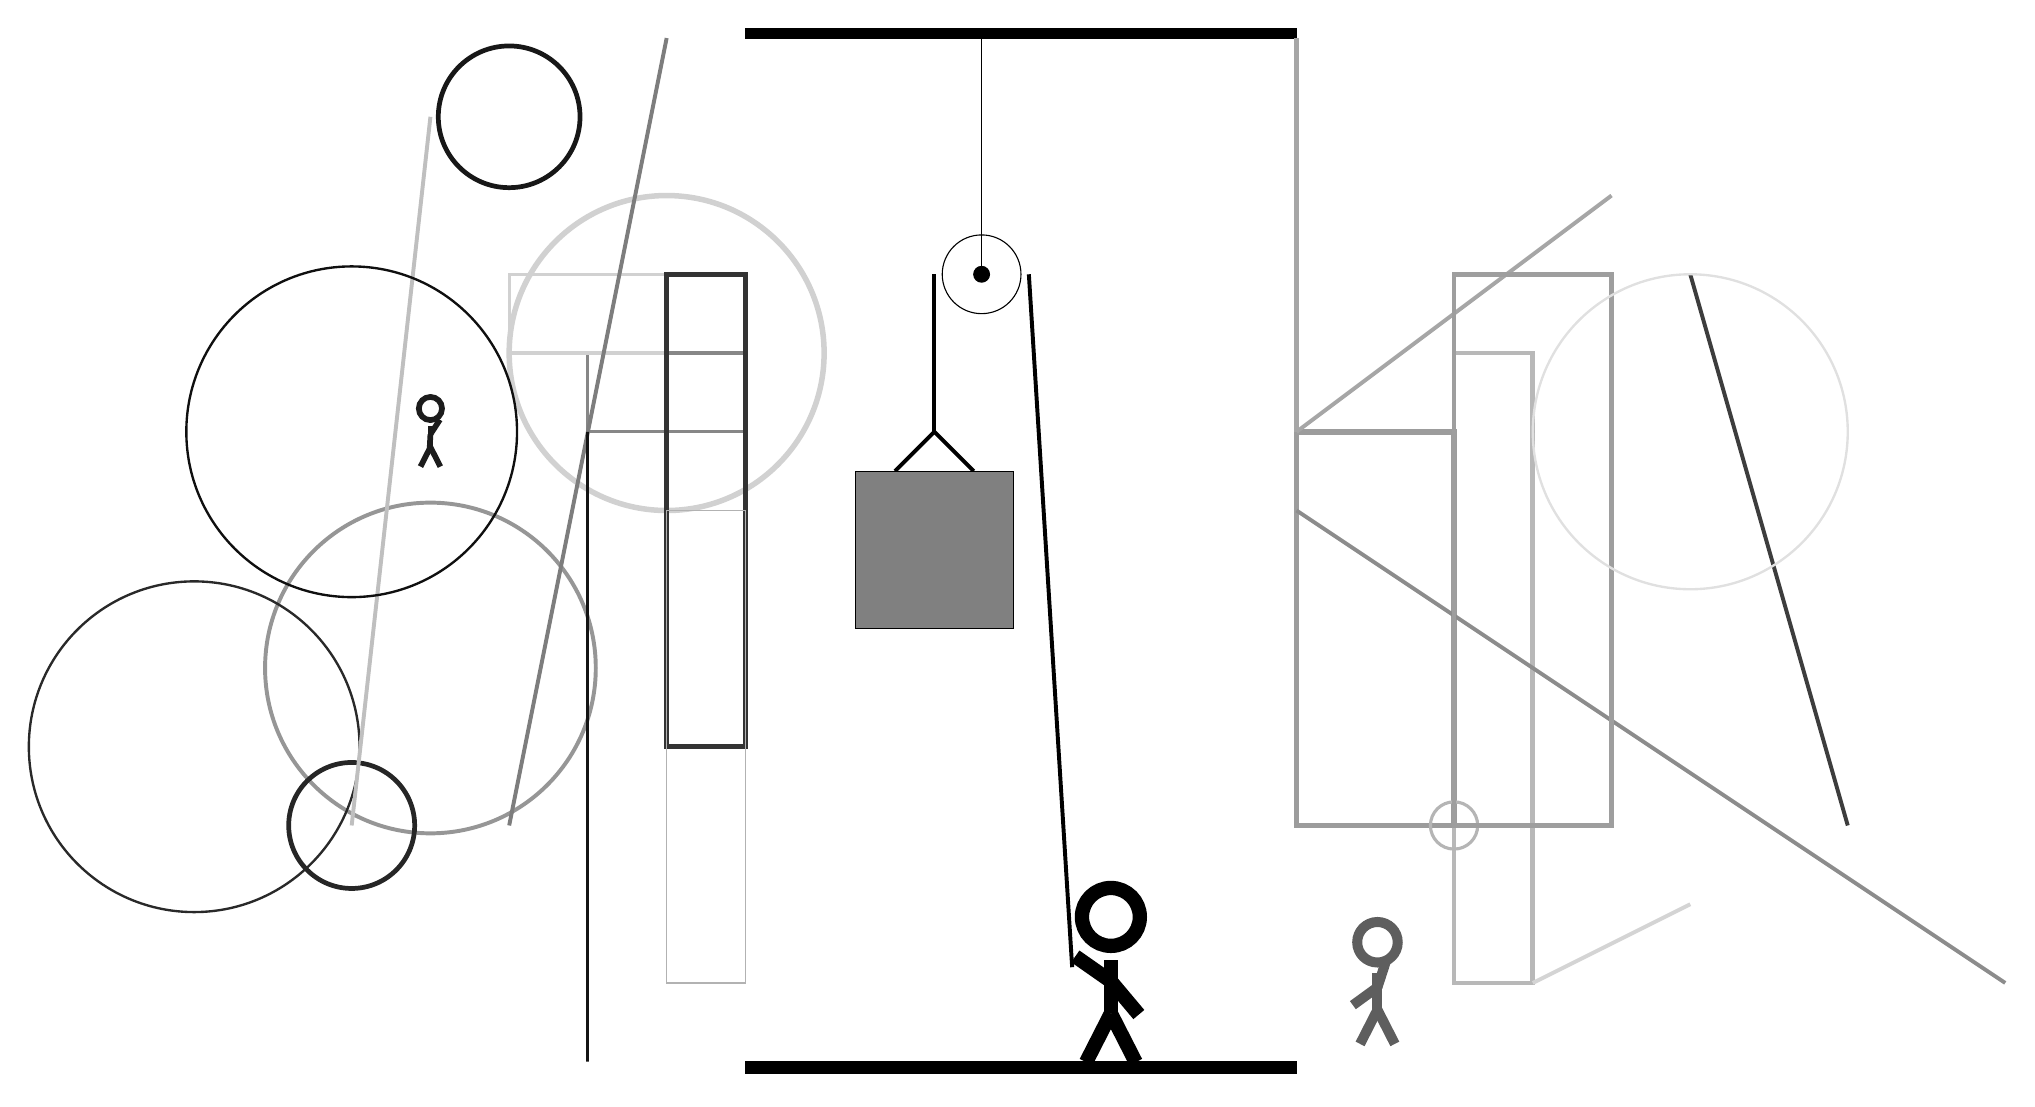
\begin{tikzpicture}
		%%%%% START %%%%%
		
		\draw[fill=black] (-2, 10) rectangle (5, 10.125);
		
		\draw (1, 7) circle (0.5);
		\draw[fill=black] (1, 7) circle (0.1);
		\draw (1, 10) -- (1, 7);
		
		\draw[line width=0.5mm] (-0.1, 4.5) -- (0.4, 5.0) -- (0.9, 4.5);
		\draw[fill=black!50] (-0.6, 4.5) rectangle (1.4, 2.5);
		
		\draw[line width=0.5mm] (0.4, 7) -- (0.4, 5.0);
		\centerarc[line width=0.5mm](1, 7)(0:180:0.6);
		\draw[line width=0.5mm](1.6, 7) -- (2.15, -1.8);
		
		\node at (2.6, -1.9) {\Strichmaxerl[10][-35][-50]};
		
		\draw [line width=0.7mm, color=black!18](-3, 6) circle (2.0);
		
		\draw [line width=0.5mm, color=black!41](-6, 2) circle (2.1);
		\draw[line width=0.6mm, color=black!28] (7, -2) rectangle (8, 6);
		\draw[line width=0.7mm, color=black!39] (5, 5) rectangle (7, 0);
		\draw [line width=0.4mm, color=black!29](7, 0) circle (0.3);
		\draw [line width=0.6mm, color=black!85](-7, 0) circle (0.8);
		\draw [line width=0.2mm, color=black!37](5, 2) circle (0.0);
		\draw [line width=0.3mm, color=black!84](-9, 1) circle (2.1);
		\draw[line width=0.5mm, color=black!35](5, 5) -- (9, 8);
		
		\draw [line width=0.6mm, color=black!91](-5, 9) circle (0.9);
		\draw[line width=0.5mm, color=black!76](10, 7) -- (12, 0);
		\draw[line width=0.5mm, color=black!45](5, 4) -- (14, -2);
		\draw[line width=0.4mm, color=black!47] (-4, 6) rectangle (-2, 5);
		
		\draw[line width=0.4mm, color=black!18] (-3, 6) rectangle (-5, 7);
		\draw[line width=0.7mm, color=black!35] (5, 5) rectangle (5, 10);
		\node[line width=0.4mm, color=black!89] at (-6, 5) {\Strichmaxerl[4][87][57]};
		
		\draw[line width=0.5mm, color=black!51](-5, 0) -- (-3, 10);
		
		\node[line width=0.7mm, color=black!63] at (6, -2) {\Strichmaxerl[7][36][72]};
		\draw[line width=0.6mm, color=black!38] (7, 0) rectangle (9, 7);
		\draw[line width=0.6mm, color=black!80] (-2, 1) rectangle (-3, 7);
		\draw[line width=0.5mm, color=black!25](-6, 9) -- (-7, 0);
		
		\draw[line width=0.2mm, color=black!30] (-3, -2) rectangle (-2, 4);
		
		\draw[line width=0.5mm, color=black!17](8, -2) -- (10, -1);
		\draw [line width=0.3mm, color=black!12](10, 5) circle (2.0);
		\draw [line width=0.3mm, color=black!94](-7, 5) circle (2.1);
		
		\draw[line width=0.4mm, color=black!92] (-4, 5) rectangle (-4, -3);
		
		
		\draw[fill=black] (-2, -3) rectangle (5, -3.15);
		
		%%%%% END %%%%%
	\end{tikzpicture}
\end{document}